% ============================================================================
% Capítulo 3 — Responsabilidade social, diversidade e acessibilidade
% ============================================================================
\section{RESPONSABILIDADE SOCIAL, DIVERSIDADE E ACESSIBILIDADE}

\subsection{Inclusão digital da agricultura familiar}

A inclusão digital não se resume ao acesso a dispositivos: envolve condições de
uso significativo da tecnologia. Na agricultura familiar, três barreiras se
somam -- conectividade instável, aparelhos de entrada e baixa familiaridade com
interfaces complexas. Uma solução que ignore essas restrições tende a ser
abandonada logo após a implantação, reproduzindo a exclusão que deveria
combater.

O AgroConecta foi projetado para operar nessas condições. O aplicativo mobile
funciona offline, armazenando localmente os lotes e as evidências até que haja
conexão; as telas utilizam linguagem direta, ícones acompanhados de texto e
formulários curtos; e o cadastro de produtores inclui o campo \emph{comunidade},
que permite reconhecer e valorizar a origem dos agricultores. O painel de
inclusão (Figura~\ref{fig:inclusao}) consolida produtores por comunidade,
situação de aprovação e percentual de telas acessíveis, transformando diversidade
em indicador de gestão.

\begin{figure}[H]
  \centering
  \caption{Painel de inclusão e diversidade}
  \label{fig:inclusao}
  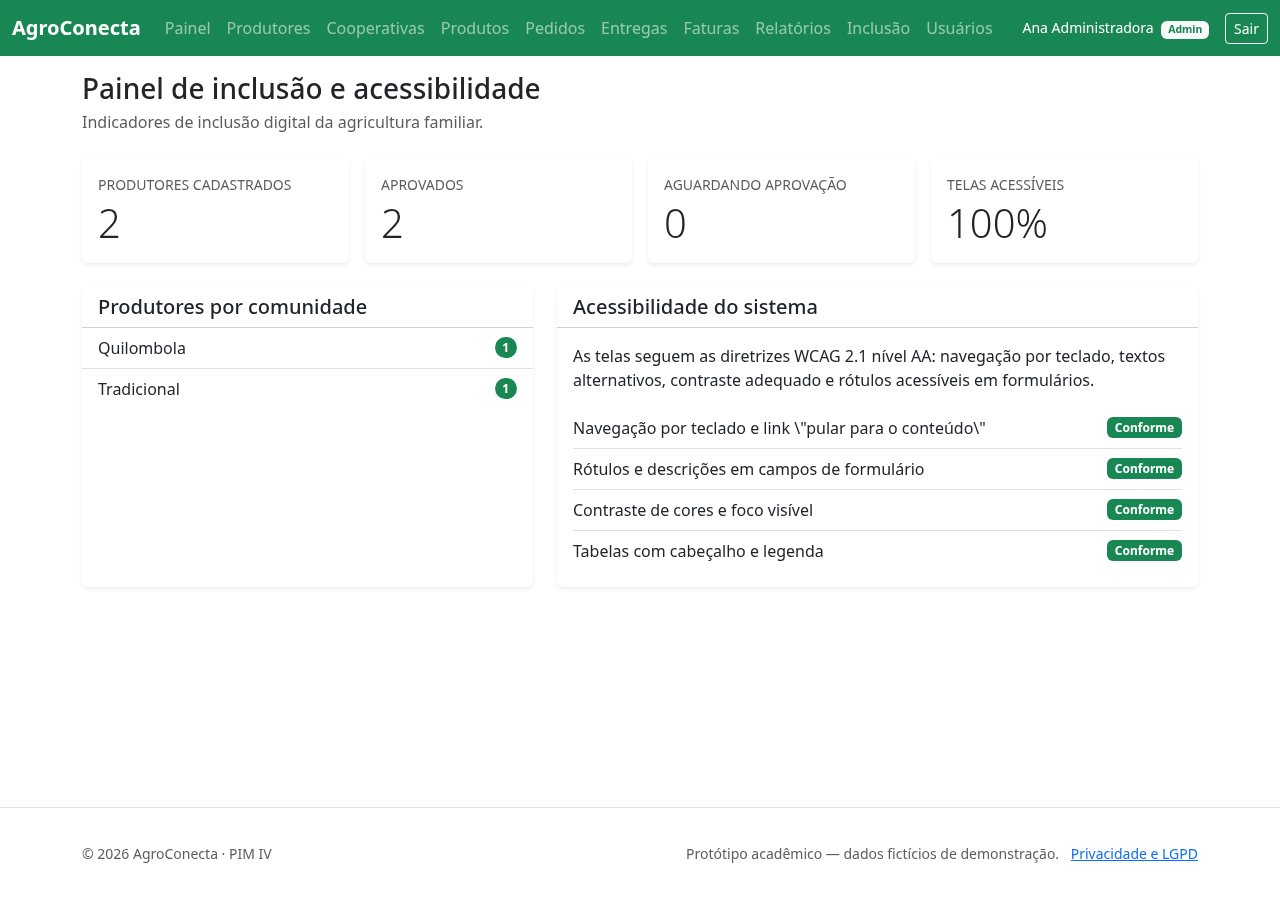
\includegraphics[width=0.92\textwidth]{figuras/inclusao.png}
  \fonte{elaborado pelo autor (2026)}
\end{figure}

\subsection{Combate à discriminação e valorização da diversidade}

O sistema adota o cadastro por comunidade -- tradicional, quilombola,
assentamento, indígena e outro -- não como mecanismo de segregação, mas de
reconhecimento e de formulação de políticas de fomento. A aprovação de cadastros
é realizada por um administrador, com registro em trilha de auditoria, o que
reduz a possibilidade de tratamento discriminatório e permite revisão das
decisões.

No plano operacional, a igualdade de acesso é garantida pelo uso em aparelhos
modestos e pela ausência de exigência de conexão permanente; no plano simbólico,
a nomenclatura e os exemplos reconhecem a contribuição das comunidades
tradicionais para a produção de alimentos.

\subsection{Acessibilidade}

As interfaces Web seguem as diretrizes WCAG 2.1 no nível AA (W3C, 2018). A
Tabela~\ref{tab:acessibilidade} relaciona os critérios aplicados e a forma de
implementação.

\begin{table}[H]
  \centering
  \caption{Critérios de acessibilidade aplicados}
  \label{tab:acessibilidade}
  \fontsize{10}{12}\selectfont
  \begin{tabular}{L{3.4cm}L{8.2cm}L{3.2cm}}
    \toprule
    \textbf{Critério} & \textbf{Implementação} & \textbf{Evidência} \\
    \midrule
    Idioma da página & Atributo \texttt{lang="pt-BR"} em todas as telas &
      Layout base \\
    Estrutura e relações & Tabelas com \texttt{caption}, \texttt{thead} e
      \texttt{scope}; formulários com rótulos associados & Telas de cadastro \\
    Contraste & Paleta com verde escuro sobre branco e foco visível &
      Folha de estilo \\
    Navegação por teclado & Ordem lógica de tabulação e link ``Pular para o
      conteúdo'' & Layout base \\
    Título da página & Título específico em cada tela & Controladores MVC \\
    Mensagens de erro & Texto descritivo junto ao campo, sem depender de cor &
      Validações \\
    Nome, função e valor & Controles nativos e \texttt{aria-label} quando
      necessário & Componentes \\
    \bottomrule
  \end{tabular}

  \vspace{2pt}
  {\fontsize{10}{12}\selectfont\itshape Fonte: elaborado pelo autor (2026), com
  base em W3C (2018)}
\end{table}

No aplicativo mobile, foram aplicados rótulos acessíveis nos botões, suporte a
escala de fonte do sistema, contraste adequado, alvos de toque com pelo menos
44 pontos e títulos semânticos de tela. A matriz de testes registra a verificação
manual com leitor de tela e as limitações encontradas, discutidas na seção 5.6.

\subsection{Proteção de dados e cidadania digital}

A plataforma trata dados pessoais de produtores, compradores e motoristas, ainda
que em contexto acadêmico e com dados fictícios. Por isso, foram adotadas medidas
alinhadas à Lei Geral de Proteção de Dados (BRASIL, 2018): finalidade e
minimização (apenas dados necessários à operação), segurança (senhas com PBKDF2,
HTTPS, autorização por papel), transparência (página pública de privacidade,
Figura~\ref{fig:privacidade}), direitos do titular (canal de contato e
possibilidade de correção) e prestação de contas (trilha de auditoria).

\begin{figure}[H]
  \centering
  \caption{Página pública de política de privacidade}
  \label{fig:privacidade}
  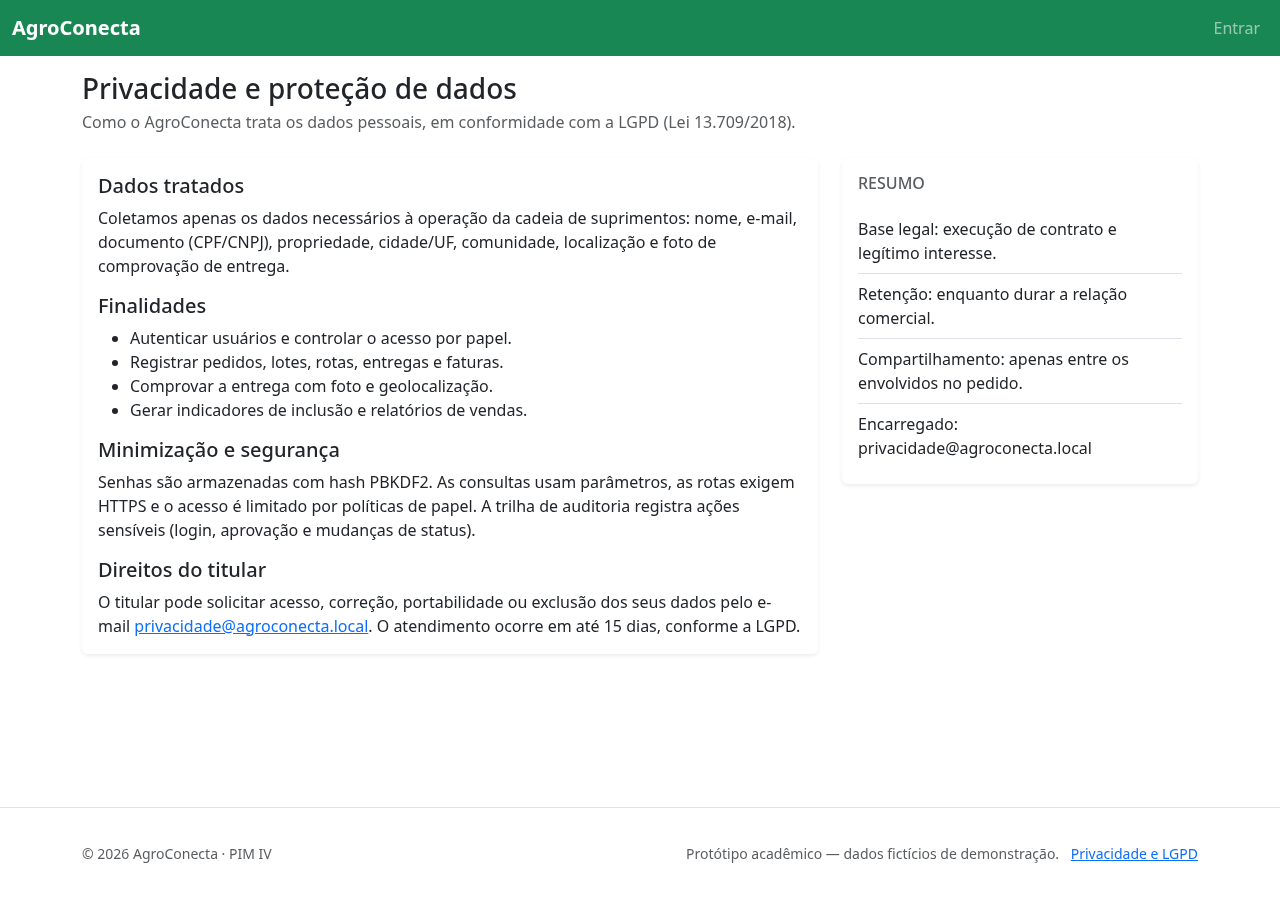
\includegraphics[width=0.92\textwidth]{figuras/privacidade.png}
  \fonte{elaborado pelo autor (2026)}
\end{figure}

\subsection{Contribuição para os Objetivos de Desenvolvimento Sustentável}

A solução dialoga com a Agenda 2030 (ONU, 2015) em três objetivos. O ODS 2
(fome zero) é apoiado pela redução de perdas e pela melhoria do escoamento da
produção. O ODS 8 (trabalho decente e crescimento econômico) é atendido pela
ampliação do acesso a mercados institucionais e pela formalização das
transações. O ODS 10 (redução das desigualdades) é endereçado pela inclusão
digital de comunidades tradicionais e pela transparência na distribuição dos
repiques financeiros entre os associados.
